\chapter{冲量和动量}

\begin{introduction}
	\item \nameref{4.1}
	\item \nameref{4.2}
	\item \nameref{4.3}
	\item \nameref{4.4}
\end{introduction}

\section{动量定理} \label{4.1}

\subsection{质点动量定理}

\begin{theorem}[质点动量定理] \label{C4-th1}
	由\nameref{C2-ax2}可得其微分形式
	
	\begin{equation}
		\dd{(m\va*{v})} = \va*{F} \dd{t} \label{C4-eq1}
	\end{equation}
	
	上式表明, \textbf{质点动量的微分等于作用在质点上合力的元冲量. }
	
	积分形式
	
	\begin{equation}
		m \va*{v}_2 - m \va*{v}_1 = \int_{t_1}^{t_2} \va*{F} \dd{t} = \va*{I} \label{C4-eq2}
	\end{equation}
	
	上式表明, \textbf{某段时间内质点动量的增量, 等于作用在质点上的合力在同一时间内的冲量. }
\end{theorem}

在直角坐标中可以写成投影式

\begin{equation}
	\begin{cases}
		m v_{2x} - m v_{1x} = \int_{t_1}^{t_2} F_x \dd{t} \\
		m v_{2y} - m v_{1y} = \int_{t_1}^{t_2} F_y \dd{t} \\
		m v_{2z} - m v_{1z} = \int_{t_1}^{t_2} F_z \dd{t} 
	\end{cases}
    \label{C4-eq3}
\end{equation}

\subsection{质点系动量定理}

质点系的动量表示为

\begin{equation}
	\va*{P} = \sum\limits_{i} m_i \va*{v}_i \label{C4-eq4}
\end{equation}

\begin{theorem}[质点系动量定理] \label{C4-th2}
	质点系动量定理的微分形式
	
	\begin{equation}
		\dd{\qty(\sum\limits_{i} m_i \va*{v}_i)} = \sum\limits_{i} \va*{F}_i \dd{t} \label{C4-eq5}
	\end{equation}
	
	上式表明, \textbf{质点系动量的微分等于作用在质点系上所有外力元冲量的矢量和. }
	
	\newpage
	
	积分形式
	
	\begin{equation}
		\sum\limits_{i} m_i \va*{v}_i - \sum\limits_{i} m_i \va*{v}_{i0} = \sum\limits_{i} \int_{t_0}^{t} \va*{F}_i \dd{t} \label{C4-eq6}
	\end{equation}
	
	上式表明, 在某段时间内, 质点系动量的增量等于作用在质点系上所有外力在同一时间内的冲量的矢量和.
\end{theorem}

质点系动量定理微分形式和积分形式也可以仿造质点动量定理写出在直角坐标中的投影形式. 

\section{质点系动量守恒定律} \label{4.2}

\begin{axiom}[质点系动量守恒定律] \label{C4-ax1}
	\begin{enumerate}
		
		\item 如果作用在质点系上所有外力的矢量和为零, 则该质点系的动量保持不变, 即
		
		\begin{equation}
			\sum\limits_{i} m_i \va*{v}_i = \overrightarrow{\text{Const}} \label{C4-eq7}
		\end{equation}
		
		\item 当作用在质点系上所有外力沿某一坐标轴投影的代数和为零时, 该质点系的动量沿同一坐标轴的投影保持不变, 即
		
		\begin{equation}
			\sum\limits_{i} m_i v_i = \text{Const} \label{C4-eq8}
		\end{equation}
		
	\end{enumerate}
\end{axiom}

\section{质心运动定理} \label{4.3}

一个物体的质心坐标$(x_c, y_c, z_c) = \qty(\dfrac{\sum m_i x_i}{M}, \dfrac{\sum m_i y_i}{M}, \dfrac{\sum m_i z_i}{M})$. 

\vskip 0.3cm

对于质量连续分布的物体, 只需把求和符号换成积分符号即可. 

\begin{theorem}[质心运动定理] \label{C4-th3}
	
	质点系的动量等于该质点系的质量与质心速度的乘积(简称质心动量). 
	
	\begin{equation}
		\sum\limits_{i} m_i \va*{v}_i = M \va*{v}_c \label{C4-eq9}
	\end{equation}
	
	质点系的质量与其质心加速度的乘积等于作用在质点系上所有外力的矢量和. 
	
	\begin{equation}
		M \va*{a}_c = \sum\limits_{i} \va*{F}_i \label{C4-eq10}
	\end{equation}
	
\end{theorem}

式(\ref{C4-eq9}), (\ref{C4-eq10})可以对三个坐标轴投影, 使用其投影式. 

\newpage

\section{第3次作业部分题目归纳} \label{4.4}

\subsection{冲量}

\begin{enumerate}
	
	\item (作业T5) 质量为$m$的质点做匀速率圆周运动, 角速度为$\omega$, 半径为$r$, 则合力在物体运动半周过程的冲量大小为 \uline{$2mr\omega$}. 
	
\end{enumerate}

\subsection{动量}

\begin{enumerate}
	
	\item (作业T7) 一系统由质量分别为$m$和$4m$的两个质点组成, 当它们以相同动能$E$沿同一直线面对面运动, 系统动量大小为 \uline{$\sqrt{2mE}$}. 
	
\end{enumerate}

\subsection{质量变化问题}

\begin{enumerate}
	
	\item (作业T17) 如图(\ref{C4-fig1})所示, 劲度系数为$k$的弹簧, 一端固定在墙上, 另一端连接一质量为$M$的容器, 容器可在光滑平面上运动, 当弹簧未变形时, 容器位于$O$点处. 今使容器自$O$点左边$l_0$处从静止开始运动, 每经过$O$点一次, 就从上方滴管中滴入一质量为$m$的油滴, 则第一滴油滴落入容器的瞬间, 容器的速率为 \uline{$(M l_0 \sqrt{k/M}) / (m + M)$}; 当容器中滴入了$n$滴油滴后, $M$容器可以偏离$O$点的最大距离为 \uline{$l_0 \sqrt{M/(M + nm)}$}. 
	
\end{enumerate}

\begin{figure}[htbp]
	\centering
	\begin{minipage}[t]{0.48\textwidth}
		\centering
		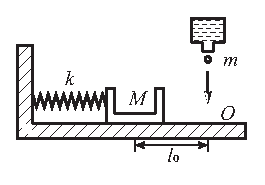
\includegraphics[scale=1.5]{C4-fig1.eps}
		\caption{作业T17题图}
		\label{C4-fig1}
	\end{minipage}
	\begin{minipage}[t]{0.48\textwidth}
		\centering
		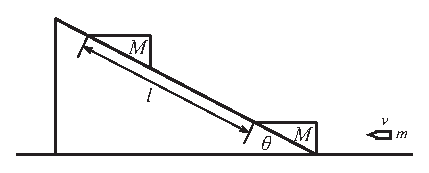
\includegraphics[scale=1.2]{C4-fig2.eps}
		\caption{作业T22题图}
		\label{C4-fig2}
	\end{minipage}
\end{figure}

\subsection{动量定理(主要是碰撞问题)}

\begin{enumerate}
	
	\item (作业T22) 如图(\ref{C4-fig2})所示, 质量为$M$的木块与表面光滑的固定斜面的底端靠在一起并处于静止状态. 一颗水平速度为$v$, 质量为$m$的子弹射向$M$木块, 并嵌入在木块内. 求嵌入了子弹的$M$木块的运动速度$V$, 以及该$M$木块可沿着光滑的固定斜面上滑的距离$l$. 
	
\end{enumerate}
